\chapter{Introduction}\label{C:intro}
\lettrine{E}{veryone} experiences the process of taking decisions during his life. As a matter of fact, drastically the life of an individual can be synthesized in its \textit{perception} of the world and its \textit{interaction} with it. The concepts of perception and interaction might seem quite straightforward to understand: for a human the perception of the world comes from its senses and the interaction comes from its possibility to change its surroundings. On the contrary, these concepts are actually absolutely hard to define and aroused, during the centuries, a strong debate between scientists, biologists, and even philosophers.

\section{Perception and interaction}
We start from the assumption that, by definition, an individual perceive the environment around it and acts on it in order to achieve \textit{goals} expressed by its will. In other words, all the actions made by an individual are done to satisfy its will to obtain something from the world it lives in. This task is naturally performed by humans, but it implies some challenging problems that are hard, or unfeasible, to solve. One of them comes from the intrinsic \textit{uncertainty} of the perception we have of the world around us. Indeed, the perception of the world consists in the interpretation of the information provided by senses, but the process of information retrieval by senses and the mental processes to understand them, inevitably introduce a certain level of noise that distorts the original true information. On the other hand, the interaction with the world deals with the will of the individual to perform actions to change the environment around it, but this apparently simple operation involves complex biologic mechanisms to coordinate the body according to the will and difficulties in the perception of the consequences of the interaction. Moreover, the concept of goal can be unclear and the individual may result in performing actions without being sure of what it wants.
It is arguable that discussing about the concept of true information and the concept of will requires strong theoretical considerations since they are both hardly definable concepts. For many centuries scientists and philosophers debated about these topics, in particular trying to solve complex problems like the real nature of perceivable things and the concept of free will. However, to make the discussion of these concepts suitable for our purposes throughout all this thesis, we lighten the definition of them to the one provided by common sense.

\section{Learn how to act with Reinforcement Learning}
\gls{rl}~\cite{sutton1998reinforcement} is a subfield of \gls{ml} which aims to realize autonomous \textit{agents} able to learn how to act in a certain \textit{environment} in order to maximize an objective function; this is achieved providing the agent with the perception of its \textit{state} in the environment and making it learn the appropriate \textit{action} to perform, where an action can be seen as an atomic operation that brings the agent from a state to another one. The objective function represents a measure of how well the agent is accomplishing its task in the environment and it is usually formalized by a discounted sum of \textit{rewards} obtained after each action (Figure~\ref{F:rl}). The sum is discounted to give more importance to the most recent rewards w.r.t. the ones further in the future. The reward function, i.e. the function returning the reward after each action, is not a concrete part of the environment, but it is often designed by a human which decides whether a certain behavior has to be reinforced (returning a positive reward) or inhibited (returning a negative reward).

\begin{figure}[t]
\begin{minipage}{\textwidth}
\begin{center}
  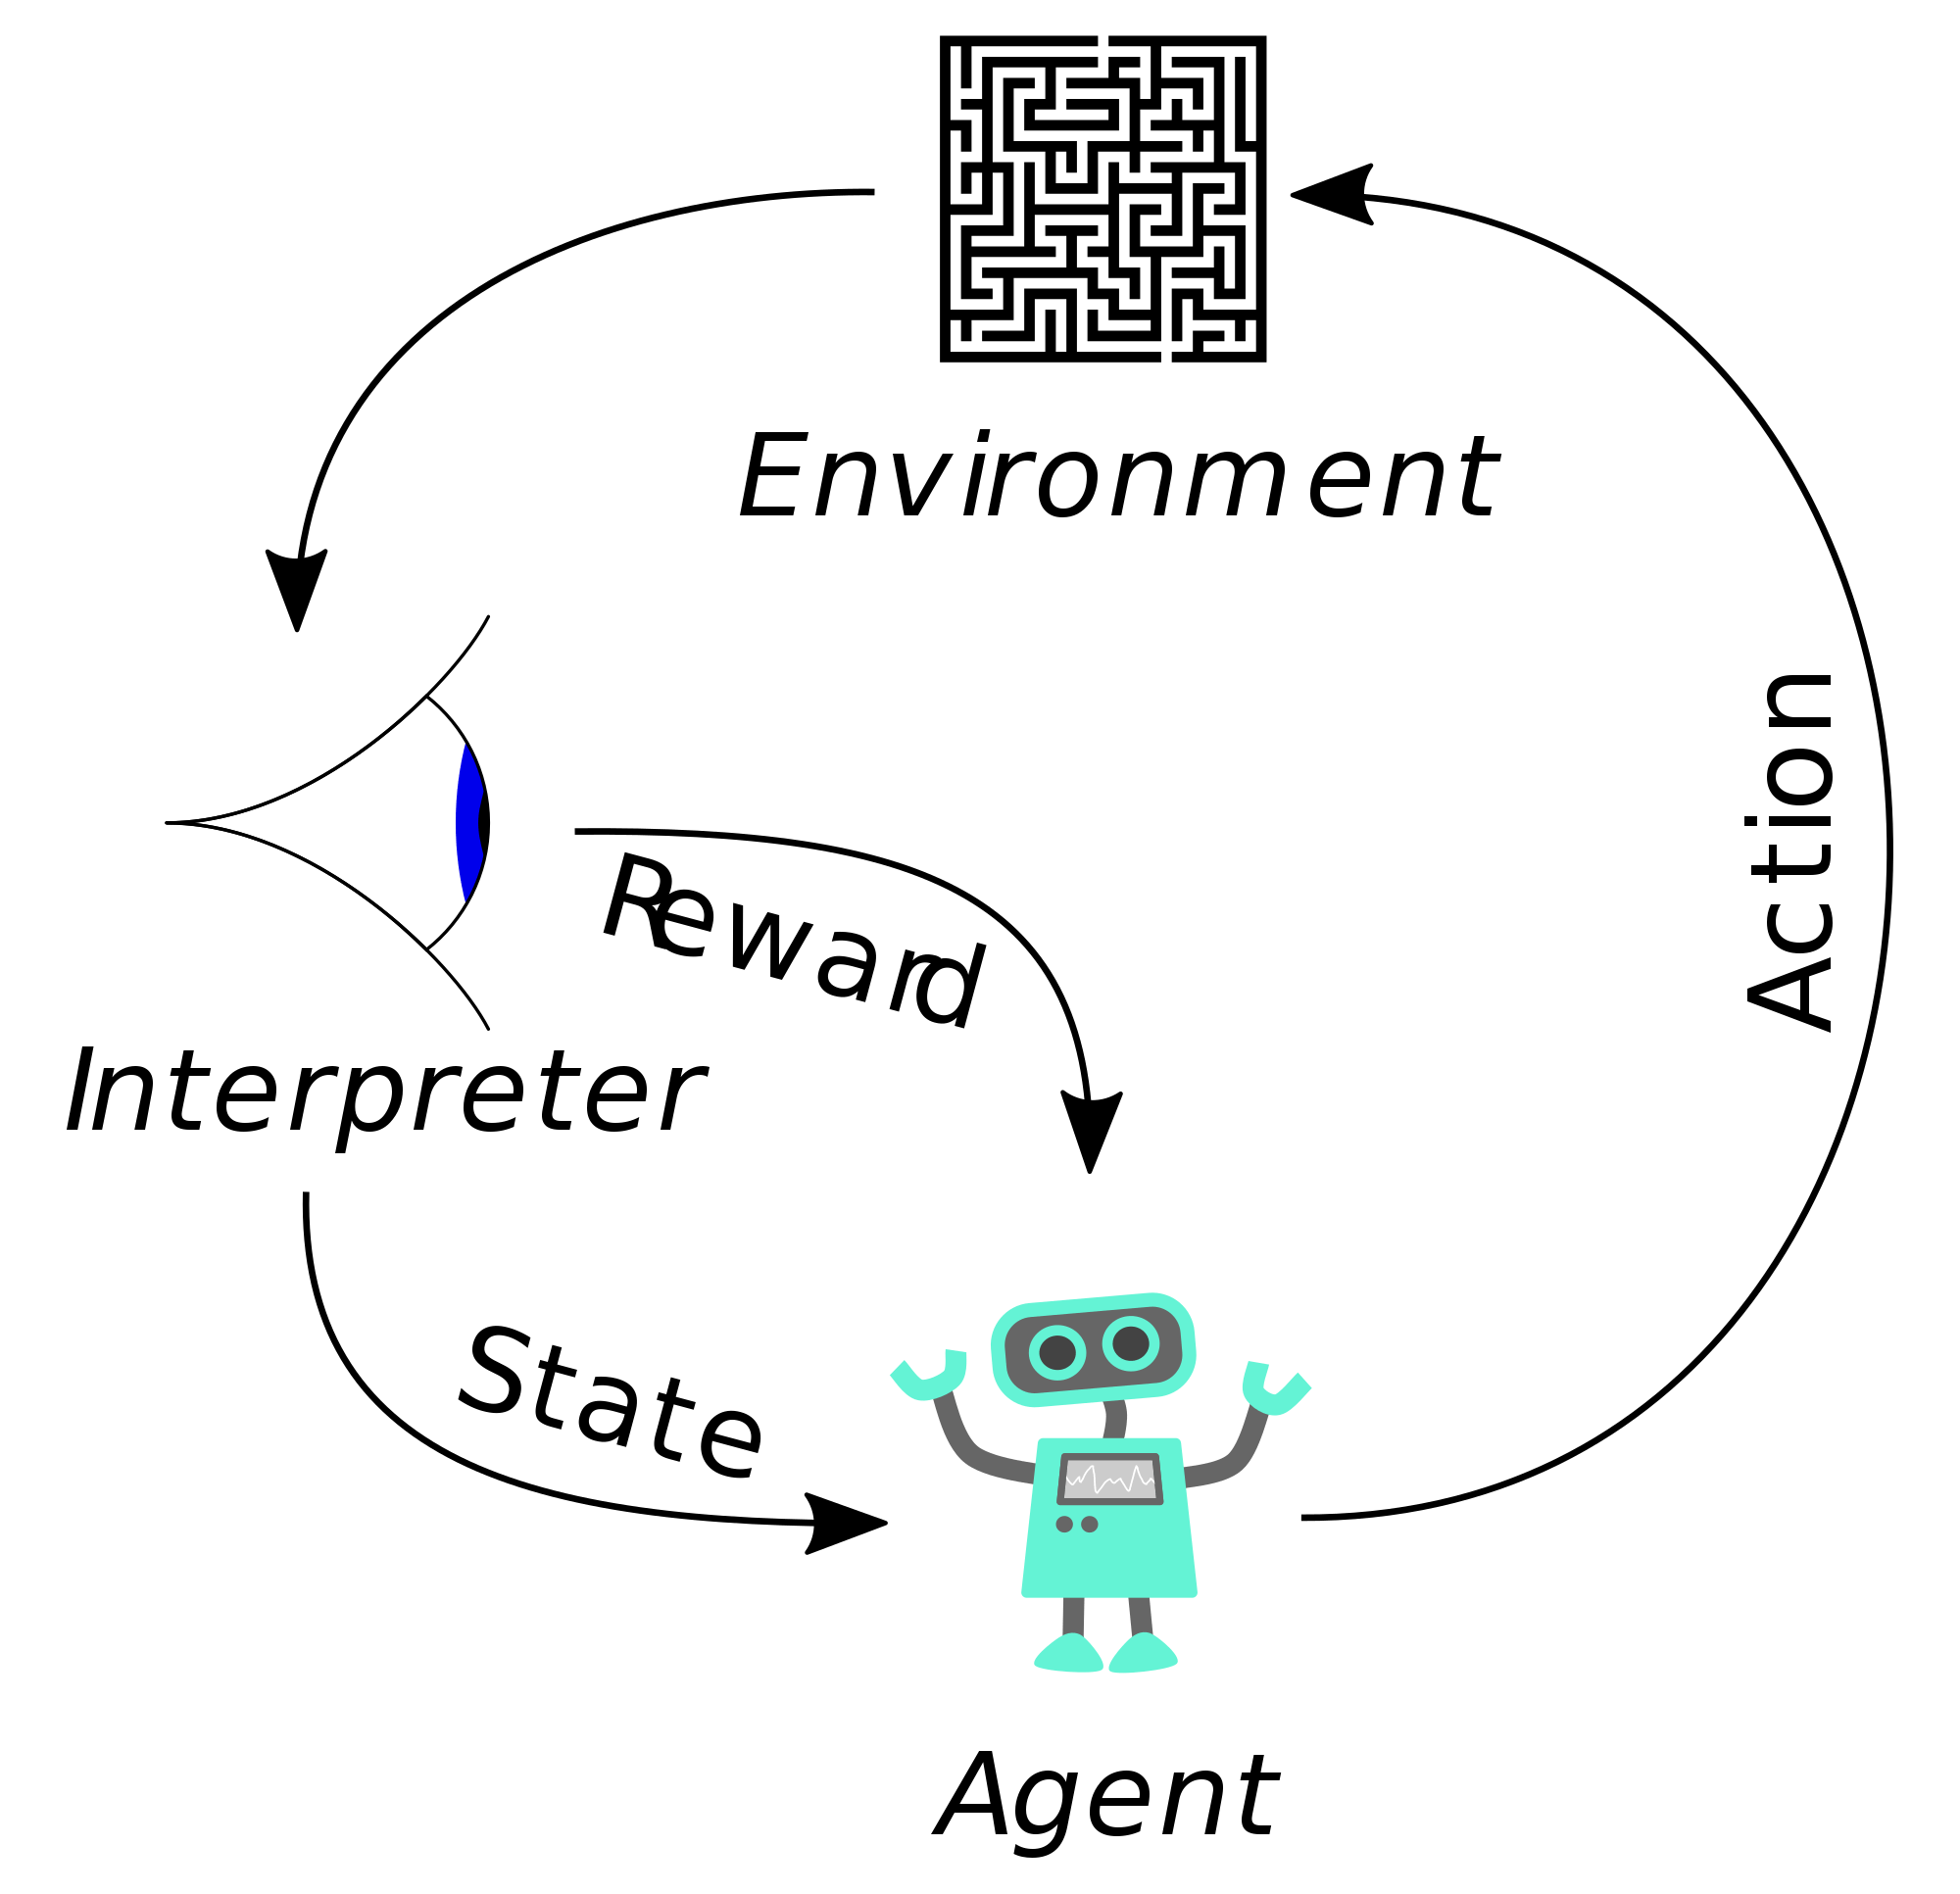
\includegraphics[scale=.1]{img/rl.png}
\end{center}
\end{minipage}
\caption[Reinforcement Learning problem scheme]{The scheme of a \gls{rl} model.}\label{F:rl}
\end{figure}

\subsection{Uncertainty in Reinforcement Learning}
The major challenge of \gls{rl} is represented by the uncertainty. In fact, initially, the agent is not provided with the knowledge of how the environment will react to its actions, thus it does not know whether an action would be good or not to maximize its objective function. In other words, before trying an action, it does not know if that action will get a positive or a negative reward, and it does not know if that action will let it go to the expected state or not. Thus, the former problem can be seen as uncertainty in the reward function and the latter as uncertainty in the transition (i.e. model) function. In some cases, also the uncertainty in the perception of the current state of the agent is considered, making the problem more complex.

The uncertainty issue results in the need of the agent to try actions in order to improve its knowledge of the environment. This process delays the collection of high rewards, but helps the agent to reduce its uncertainty. However, since the objective function is a sum of discounted rewards where later rewards worth less than recent ones, the agent also needs to learn fast in order to learn to perform the most rewarding actions as soon as possible. The need to \textit{explore} to reduce uncertainty and the need to \textit{exploit} the actions believed to be good introduces an important problem known as \textit{exploration-exploitation dilemma}.

\subsection{Balancing exploration and exploitation}
The exploration-exploitation dilemma has been broadly studied in the field of \gls{mab}, a particular case of the \gls{rl} problem with a single state~\cite{lai1985asymptotically}. In this problem the goal is to find the sequence of optimal actions, i.e. the sequence of actions that allows to maximize the return. The simplistic setting of the \gls{mab} problem allows to theoretically study the balancing of exploratory and exploitative actions, for instance to derive upper confidence bounds on the \textit{regret}, i.e. a measure of the return lost in performing non-optimal actions~\cite{bubeck2012regret, agrawal2012analysis, vermorel2005multi}, and several algorithms to address this problem have been proposed such as UCB1~\cite{auer2002finite} and Thompson Sampling~\cite{thompson1933likelihood}.

The \gls{rl} setting complicates the \gls{mab} problem because of the presence of multiple states. This makes the exploration-exploitation dilemma less tractable in terms of complexity and computational feasibility. Indeed, the quality of the actions must now be evaluated for each state, contrarily to the \gls{mab} case where the presence of a single state simplifies the problem. This issue is what makes \gls{rl} so challenging and has been addressed for decades in the literature.

\section{My research}
The strong connection between uncertainty and the exploration-exploitation dilemma is highlighted by the previous considerations and it is intuitive how the effectiveness of a \gls{rl} algorithm depends on its ability of reducing the uncertainty of the agent in a computationally and data-efficient way. The \gls{rl} literature contains lots of algorithms and methodologies proposed to make the agent learn a good policy aiming at efficiency; however, despite addressing the reduction of uncertainty via experience, only few of them explicitly exploit uncertainty to learn.

\subsection{What is my research about}
During my Ph.D., I studied ways to develop algorithms that exploit uncertainty since the explicit consideration of uncertainty has been shown to be often helpful in order to improve the performance and efficiency of learning. One of the most common technique to explore is known as $\varepsilon$-greedy and consists in performing, at each state, a random action with probability $\varepsilon$ and the action considered to be the best one with probability $1 - \varepsilon$. This exploratory policy does not consider the uncertainty of the agent and simply randomly moves it with the drawback of requiring a huge amount of experience to learn effective policies. This is shown especially in recent works on the field of \gls{drl}~\cite{mnih2015human, van2016deep, wang2015dueling} which studies the application of \gls{dl} models and methodologies to exploit their strong ability to generalize with the purpose to solve highly complex problems that were unfeasible before. Research on \gls{drl}, brought to the realization of groundbreaking works where authors have been able to reach the state-of-the-art in extremely complex games such as Go~\cite{silver2016mastering, silver2017mastering} and chess~\cite{silver2017chess}.
However, the extraordinariness of these results is comparable to the amount of experience required by these algorithms to work. For instance, in~\cite{mnih2015human} the experiments are performed using $50^6$ samples corresponding to three days of computation and several weeks of human play. This work does not address the problem of data-efficiency aiming more to other goals (e.g. maximizing the cumulative reward) and for this reason the previously described exploration policy of $\varepsilon$-greedy is used.

\subsection{What I have done}
My Ph.D. research brought to the publication of four conference papers, most of them focused on the previously described topic. I also developed, together with a colleague of mine, a \gls{rl} Python library called \textit{Mushroom} which had the initial purpose to facilitate my research, but which has become larger and larger allowing now to do \gls{rl} research for general purposes. Details about Mushroom are reported in Appendix~\ref{App:msh}. Other works are still ongoing and others have not been accepted for publications yet, still I think they worth to be mentioned in this thesis anyway. The whole document is divided in four parts, with this introduction included in the first one:
\begin{itemize}
 \item \textbf{first} part includes this chapter and Chapter~\ref{C:soa} which introduces the main concepts of \gls{rl} starting from the fundamental theory and then giving a description of several methodologies related to this thesis with the purpose to provide a general, but useful, overview of what is necessary to understand the following chapters;
 \item \textbf{second} part includes the description of three publications I made about ways to exploit uncertainty in the context of Value-Based \gls{rl} and more in particular in the famous algorithm of $Q$-Learning. In particular, Chapter~\ref{C:mev} describes a novel way to address the problem of overestimation of the Maximum Expected Value in $Q$-Learning and Chapter~\ref{C:rq} describes a novel way to deal with uncertainty in the estimate of the components of the Bellman Operator;
 \item \textbf{third} part includes two works about the exploitation of uncertainty to drive exploration. Chapter~\ref{C:ts} describes a set of algorithms for the estimate of uncertainty of action-values to allow the use of an exploration policy inspired by Thompson Sampling. Chapter~\ref{C:opt} introduces a variant of the Bellman Operator which incorporates an optimistic update of the action-value estimate in order to favor exploration according to the principle of Optimism in the Face of Uncertainty;
 \item \textbf{fourth} and last part concludes the thesis resuming the previous chapters and giving my considerations about the research I made and the one I think will be interesting to pursue in the following years, by me or someone else!
\end{itemize}
